\begin{tikzpicture}
	\pgfplotsset{/tikz/font={\footnotesize}}
	\begin{axis}[
			% xlabel={Additional $8\times8$ transforms},
			ylabel={Y BD-rate (\%)},
			grid=both,
			scale only axis,
			width=0.8\textwidth,
			height=0.225\textheight,
			xtick={0, 1, 2, 4, 8, 16},
			x tick label style={
				rotate=-45, anchor=west,
				/pgf/number format/.cd,
				fixed,
				fixed zerofill,
				precision=0,
			},
			% xticklabels={0, 1, 2, 4, 8, 16, 32},
			ytick={0,-1,-2,-3,-4,-5,-6},
			% yticklabels={0\%, -1\%, -2\%, -3\%, -4\%, -5\%, -6\%},
			xmin=0, xmax=16,
			ymin=-3, ymax=0,
			% legend entries={sep-$8\times8$,nsep-$8\times8$},
			legend style={nodes=right},
			legend pos= north east,
            xticklabels={DST, DST + 1 RDOT, DST + 2RDOT, DST + 4 RDOT, DST + 8 RDOT,
			DST + 16 RDOT},
		]

		% \pgfplotstableread{figures/prog_transf_8x8.dat}\table
		% \addplot[mark=*,mark size=1.1pt, red, thick, smooth, tension=0.3, dashed]
		% table[x=ntrans,y=sep,col sep=tab] from \table;

		\addplot [mark=*,mark size=1pt, red, thick, dashed] table {
		0	0
		1	-0.79
		2	-1.06
		4	-1.28
		8	-1.42
		16	-1.54
		};
		\addlegendentry{Separable}

		\addplot [mark=*,mark size=1pt, red, thick] table {
		0	0
		1	-1.75
		2	-2.09
		4	-2.28
		8	-2.34
		16	-2.44
		};
		\addlegendentry{Non-separable}
	\end{axis}
\end{tikzpicture}

% vim:set filetype=tex:
